\documentclass[memoire.tex]{subfiles}

\begin{appendices}

\chapter{Les différents concepts du Big Data}

\section{Architecture Réactive}
\label{a:architecture-reactive}

Le nombre de données augmentant très rapidement et les clients demandant un service le plus rapide possible et disponible à tout moment, il est de ce fait important d'avoir une infrastructure facilement adaptable à ce flux. C'est le but de l'architecture réactive~\cite{ARCH_REACTIVE}.
Elle repose sur quatre principes : 
\begin{figure}[!h]
	\centering 
	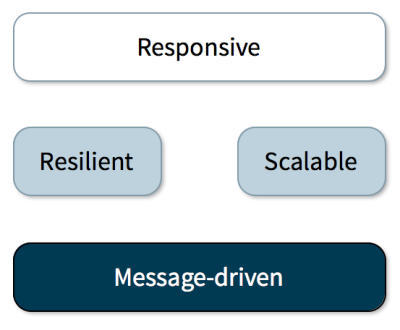
\includegraphics[scale=0.48]{img/arch-reactive.png}
	\caption{Schéma de l'architecture réactive}
	\label{Architecture réactive}
\end{figure}
\begin{itemize}
\item Responsive : C'est l'objectif à atteindre.
\item Scalable et Resilient : L'objectif ne peut pas être atteint sans remplir ces deux conditions.
\item Message Driven : C'est la base qui permettra d'accueillir tous les composants afin d'obtenir une architecture réactive
\end{itemize}


\textbf{Responsive} :
Un système responsive doit être en mesure de réagir rapidement à toutes les requêtes peut importe les circonstances, dans le but de toujours fournir une expérience utilisateur positive.
La clé afin de proposer ce service, est d'avoir un système élastique et résilient, les architecture "Message Driven" fournissent les bases pour un système réactif.
L'architecture Message Driven est aussi important pour avoir un système responsive, parce que le monde fonctionne de manière asynchrone tout comme elle. Voici un exemple : Vous voulez vous faire du café, mais vous vous rendez compte que vous n'avez plus de crème et de sucre.

Première approche :
\begin{itemize}
\item Mettre du café dans votre machine.
\item Aller faire vos courses pendant que la machine fait couler le café.
\item Acheter de la crème et du sucre.
\item Rentrer chez vous.
\item Boire votre tasse de café.
\item Profiter de la vie !
\end{itemize}

Seconde approche :
\begin{itemize}
\item Aller faire vos courses.
\item Acheter de la crème et du sucre.
\item Rentrer chez vous.
\item Mettre du café dans votre machine.
\item Regarder impatiemment la cafetière se remplir.
\item Expérimenter le manque de caféine.
\item Et enfin, boire votre tasse de café.
\end{itemize}

Grâce à la première approche, on peut clairement voir la différence de gestion de l'espace et du temps. C'est grâce à cela que cette architecture est un atout primordiale pour assurer un système responsive.


\textbf{Resilient} :

La plupart des applications sont conçus par rapport à un fonctionnement idéal. C'est à dire qu'elle ne prévoient pas de gérer correctement les erreurs qui peuvent intervenir plus souvent que ce qu'on pourrait croire. Cela à pour effet de na pas garantir une disponibilité continu et peut provoquer la perte de crédibilité d'un service. La résilience est là pour pallier à ce problème, elle à pour but de récupérer les erreurs émises et de les traiter correctement afin de ne pas provoquer d'interruption de service et de ne pas impacter l'expérience utilisateur.


\textbf{Scalable} :

La résilience et l'élasticité vont de pair dans la construction d'une architecture réactive. L'élasticité permet d'adapter facilement le système à la demande et d'assurer sa réactivité peu importe la charge qu'il subit. L'élasticité est un point très important, lorsque votre plateforme reçoit énormément de connexion cela veut dire que votre service connaît un succès important, c'est donc le pire moment pour avoir un service non disponible. Cela entrainerait une perte de crédibilité et de clients.

Il existe deux moyens différents de rendre élastique une application : 
\begin{itemize}
\item La mise à l'échelle verticale
\item La mise à l'échelle horizontale (Architecture Répartie)
\end{itemize}

La mise à l'échelle verticale consiste à maximiser l'utilisation des ressources de notre machine. Cela peut se faire par l'utilisation de programmes fonctionnant en asynchrone sur plusieurs threads. Tandis que la mise à l'échelle horizontale consiste à augmenter le nombre de machine afin d'avoir plus de ressources à notre disposition. Pour le moment on ne vas pas trop s'attarder sur la division horizontale car une partie lui est dédiée.

La mise à l'échelle verticale est certes la moins couteuse, mais ce n'est pas la plus simple à mettre en place. En effet le multithreading permet de tirer la maximum des performances de la machine, mais cela ajoute une certaine complexité au programme. Par exemple le fait de travailler avec des variables mutables entre différents threads n'est pas une tâche aisée, cela provoque donc des limitations à la mise à l'échelle verticale. De plus, une fois avoir exploiter au maximum une machine en ayant mis en place la mise à l'échelle verticale, si on a encore besoin de ressources supplémentaire la mise à l'échelle horizontale devient indispensable.

\textbf{Message-Driven} :

Le Message-Driven Architecture est la base d'une architecture réactive. Une application dirigée par message peut être dirigée par des évènements, par des acteurs ou par les deux.

Un système déclenché par événement est basé sur des événements qui sont surveillés par zéro observateur ou plus. Les évènement ne pointent pas directement vers une destination en particulier, ils sont écoutés et les entités qui écoutent les évènements vont interagir lorsque qu'ils en ont détecter un.

Un système dirigé par des acteurs est une extension de l'architecture de transmission de messages. Les messages sont envoyés à des destinataires précis, appelés acteurs. Les messages sont envoyés dans la boite aux lettres des acteurs, et seront traités dès que l'acteur aura du temps.

\section{Architecture Répartie}
\label{a:architecture-repartie}


Une architecture répartie ou bien un système distribué représente tout simplement une mise à l'échelle verticale. C'est à dire un groupe de machines travaillant ensemble, mais en donnant l'impression que ce n'est qu'une seule machine.

Ces machines ont un état partagé, elles fonctionnent simultanément et peuvent tomber en panne indépendamment sans perturber le fonctionnement du reste du système. Cela peut permettre notamment d'attribuer facilement plus de ressource à une application lors d'une montée en charge.

\end{appendices}